% !TEX root = template.tex

\section{Related Work}
\label{sec:related_work}

Activity recognition is a field evolving for more than twenty years, it started from very simple motion recognition and it gets more complex over the years.
As just said, the classical approach to this problem is with a feature extraction techniques.
In these solutions, ad-hoc features are extracted from the dataset, reducing the dimension of each signals from the recorded sample to a feature vector.
In this way features can be classified using several classifiers to obtain an accurate prediction.

\begin{figure}[!ht]
  \centering
  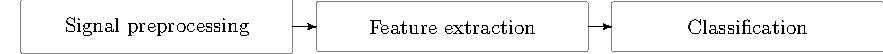
\includegraphics[width=\linewidth]{feature_extraction}
  \label{fig:feature_extraction}
  \caption{Processing pipeline for feature extraction techniques}
\end{figure}

The main processing pipeline used from these solutions is reported in \fig{fig:feature_extraction}.
The most used classifiers for feature extraction are Decision Trees, \gls{svm}, K-nearest neighbors and Naive Bayes although a lot of different classifiers can be used ~\cite{Ravi05}.
Features can be extracted either from a single sensor or from a large set of sensors, the first solution suffers an high computational complexity while the second is computational easier but certainly less  portable and can create issues due to redundancy of the information.
In ~\cite{Laerhoven02} they collect data from 30 sensors positioned around the body and they classify features extracted from these data with a clustering algorithm. They chose to collect all the data in a central processing unit to perform a centralized classification. This approach suffers however an high cost and an high complexity to limit redundancy in the data.

The problem of this technique is the strong data dependence even if it gets a good accuracy.

To overcome this lack of the classical \gls{ars}, deep learning is used in several ways.
In ~\cite{Chikhaoui17} the authors perform a matrix factorization for dimensionality reduction and deep learning algorithm to automatically learn suitable features.
In this work, they reduce the dimension of the dataset using matrix factorization and they elaborate the results in a Neural Network. The output of the \gls{nn} is a feature vector. Finally the activity is predicted classifying the feature vector with a Softmax classifier.
The accuracy is quite good since they avoid hand-crafted features, but they still rely on features extracted from data.

The key to implement an adaptable and reliable algorithm to classify human activities is the use of deep learning without extracting features at all.
A comparison between three different deep learning algorithms is made in ~\cite{Xu2017}. They collected data from one single sensor and they predicted activities using \gls{dt}, \gls{ann} and \gls{rf}. They stated that \gls{rf} performs better than the other two, with an accuracy between $75 \%$ and $90 \%$ depending on the activity.


\MR{The goal of this section is to describe what has been done so far in {\it the} literature. You should focus on and briefly describe the work done in the best papers that you have read. For each you should comment on the paper's contribution, on the good and important findings of such paper and also, 1) on why these findings are not enough and 2) how these findings are improved upon / extended by the work that you do here. At the end of the section, you recap the main paper contributions (one or two, the most important ones) and how these extend / improve upon previous work. If possible, I would make this section no longer than one page, this leads to an overall {\it two pages} including abstract, introduction and related work. I believe this is a fair amount of space in most cases.}\\
\begin{itemize}
\item \MR{\textbf{References:} please follow this {\it religiously}. It will help you a lot. Use {\it bibtex} as the tool to manage the bibliography. A bibtex example file, maned {\tt biblio.bib} is also provided with this package.}

\item \MR{When referring to \textbf{conference / workshop papers}, I recommend to always include the following information: 1) author names, 2) paper title, 3) conference / workshop name, 4) conference / workshop address, 5) month, 6) year. Examples of this are: \cite{Zargham-2011}\cite{Sadler-2006}.}

\item \MR{When referring to \textbf{journal papers}, include the following information: 1) author names, 2) paper title, 3) full journal name, 4) volume, 5) number, 6) month, 7) pages, 8) year. Examples of this are: \cite{Shannon-1948}\cite{Boyd-2011}\cite{Zordan-2014}.}

\item \MR{For \textbf{books}, include the following information: 1) author names, 2) book title, 3) editor and edition, 4) year.}
\end{itemize}
%
\MR{Note that some of the above fields may not be shown when you compile the Latex file, but this depends on the bibliography settings (dictated by the specific Latex style that you load at the beginning of the document). You may decide to include additional pieces of information in a given bibliographic entry, but please, be consistent across all the entries, i.e., use the same fields. Exceptions are in the (rare) cases where some of the fields do not exist (e.g., the paper {\it number} or the {\it pages}).}